%   Filename    : chapter_4.tex 
\chapter{Preliminary Results/System Prototype}
The main goal of this study is to develop a system through the use of speech recognition to assess the reading miscues of the speaker. In order to achieve that goal, Kaldi, a toolkit for speech recognition, is used to develop a model in speech processing. 

\begin{figure}
    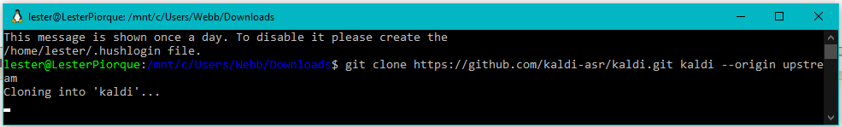
\includegraphics[width=\linewidth]{sp-install-0.png}
    \caption{Installation of Kaldi}
    \label{fig:1}
  \end{figure}

The data needed for this paper are the audio files from three different speakers. A total of 15 audio files are made. Each speaker has five Hiligaynon words to say. Two speakers are assigned to the training data and one speaker for the testing data.
Kaldi is made for an ubuntu operating system. Most of the members of this paper have windows OS on their machines. A virtual machine intended for the Ubuntu environment cannot withstand the requirements and installation needed by the toolkit to perform its operation. Also, a high-end GPU is needed in order to have successful modeling. The group has reached the stage of testing the model, but errors have been shown right after running the testing file. Hopefully, in the next test, we can successfully run the model and have some conclusions and decisions regarding the result of the process.

\begin{figure}
	\centering
	\begin{subfigure}[b]{0.3\textwidth}
		\centering
		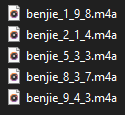
\includegraphics[width=\textwidth]{sp-audio-0.png}
		\caption{Audio files for Speaker Benjie}
		\label{fig:y equals x}
	\end{subfigure}
	\hfill
	\begin{subfigure}[b]{0.3\textwidth}
		\centering
		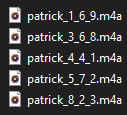
\includegraphics[width=\textwidth]{sp-audio-1.png}
		\caption{Audio files for Speaker Patrick}
		\label{fig:three sin x}
	\end{subfigure}
	\hfill
	\begin{subfigure}[b]{0.3\textwidth}
		\centering
		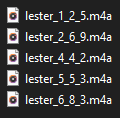
\includegraphics[width=\textwidth]{sp-audio-2.png}
		\caption{Audio files for Speaker Lester}
		\label{fig:five over x}
	\end{subfigure}
	\caption{Audio files}
	\label{fig:audio-files}
\end{figure}